\section{符号约定}

\subsection{分数幂奇函数}
本文常用的符号为符号函数和sig 函数,对于标量,其几何意义为符号函数,对于标量其定义为:
\begin{equation}
    \sig{x}^0=\sgn{x}=\begin{cases}
    	1   & x>0\\
    	-1 & x<0\\
    	0  & x=0\\
    \end{cases}
\end{equation}
基于此,我们定义$\sig{x}^q=|x|^q \sgn{x}$.

类似的,相关定义可以拓展到向量形式,其几何意义为向量$\vec{x}$的单位向量:
\begin{equation}
	\sig{\vec{x}}^0=\sgn{\vec{x}}=\begin{cases}
		\frac{\vec{x}}{\norm{\vec{x}}}, & \norm{\vec{x}}\neq 0\\
		\vec{0}   & \norm{\vec{x}}=0
	\end{cases}
\end{equation}
基于此,我们定义$\sig{\vec{x}}^q=\|\vec{x}\|^q \sgn{\vec{x}}$.

下面介绍对几个常见的求导运算,使用多维向量的情况。
\begin{equation}
	\frac{\dd}{\dd t} \norm{\vec{x}}
	= \frac{\dd}{\dd t} \sqrt{\vec{x}^T\vec{x}}
	= \frac12 \frac{1}{\sqrt{\vec{x}^T\vec{x}}}\frac{\dd}{\dd t} {\vec{x}^T\vec{x}}
	= \frac12 \frac{1}{\sqrt{\vec{x}^T\vec{x}}} (2 \vec{x}^T \dot{\vec{x}})
	= \frac{\vec{x}^T\dot{\vec{x}}}{\norm{\vec{x}}}
\end{equation}
\begin{equation}
	\frac{\dd}{\dd t} \sig{\vec{x}}^q
	=\frac{\dd}{\dd t} \norm{\vec{x}}^{q-1} \vec{x}
	=\norm{\vec{x}}^{q-1} \dot{\vec{x}}+(q-1) \norm{\vec{x}}^{q-2}  \frac{\vec{x}^T\dot{\vec{x}}}{\norm{\vec{x}}}\vec{x}
\end{equation}
也就是说这里是基于向量的定义是难以求导的,这给一些从标量系统到向量的分析带来了困难。
\begin{equation}
	\frac{\dd}{\dd t} \sig{x}^q
	=|x|^{q-1} \dot{x}+(q-1) |x|^{q-2}  \frac{x \dot{x}}{|x|}x
	=q|x|^{q-1}\dot{x},
\end{equation}


\begin{figure}
	\centering
	\begin{tikzpicture}
		\draw[->] (-2.2,0) -- (2.2,0) node[right] {$x$};
		\draw[->] (0,-1.8) -- (0,2.2) node[above] {$y$};
		\draw[domain=0:1.3,smooth,variable=\x,blue] plot ({\x},{\x*\x}); 
		\draw[domain=-1.3:0,smooth,variable=\x,blue] plot ({\x},{-\x*\x}); 
		\node[blue] at (2,2) {$y_1=\sig{x}^2$};
		\draw[domain=0:1.4,smooth,variable=\x,cyan] plot ({\x},{sqrt(\x)}); 
		\draw[domain=-1.4:0,smooth,variable=\x,cyan] plot ({\x},{-sqrt(-\x)}); 
		\node[cyan] at (2.4,1) {$y_2=\sig{x}^{1/2}$};
	\end{tikzpicture}
	\quad
	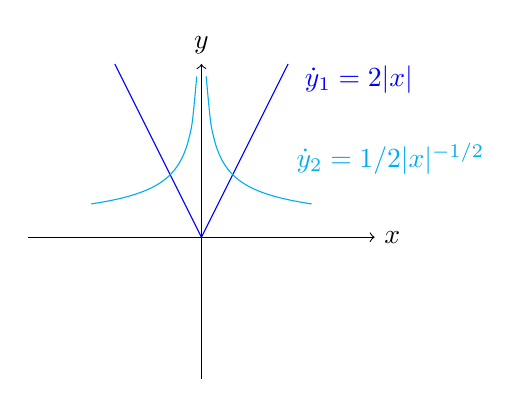
\begin{tikzpicture}
		\draw[->] (-2.2,0) -- (2.2,0) node[right] {$x$};
		\draw[->] (0,-1.8) -- (0,2.2) node[above] {$y$};
		\draw[domain=0:1.1,smooth,variable=\x,blue] plot ({\x},{2*\x}); 
		\draw[domain=-1.1:0,smooth,variable=\x,blue] plot ({\x},{-2*\x}); 
		\node[blue] at (2,2) {$\dot{y}_1=2|x|$};
		\draw[domain=0.06:1.4,smooth,variable=\x,cyan] plot ({\x},{1/2*1/sqrt(\x)}); 
		\draw[domain=-1.4:-0.06,smooth,variable=\x,cyan] plot ({\x},{1/2*1/sqrt(-\x)}); 
		\node[cyan] at (2.4,1) {$\dot{y}_2=1/2|x|^{-1/2}$};
	\end{tikzpicture}
	\caption{两个分数幂函数及其导数}
\end{figure}
